%-----------------------
% Title page
%-----------------------
\begin{titlepage}
  \centering

  \textsc{ELEC4630 Assignment 2}\\
  \vspace{9cm}

  \rule{\linewidth}{0.5pt}\\

  \vspace{1em}
  \LARGE\textsc{Question 2}\\
  \vspace{1em}

  \LARGE\uppercase{\textbf{{3D Reconstruction}}}\\

  \rule{\linewidth}{2pt}\\

  \vfill

  \normalsize{Deren Teo (4528554)}
  \vspace{1cm}

\end{titlepage}

%-----------------------
% Report body
%-----------------------
\section{Introduction}

Dense 3D reconstruction from multiple RGB images has long been a topic of interest in computer vision, and serves numerous practical purposes \cite{ulusoy_2016}. For example, 3D reconstruction applied to medical imaging can enable medical experts to better visualise areas of interest, for more accurate dianoses and better planning of medical procedures \cite{icoi_nd}. 3D reconstruction also has applications in a civil engineering context, to reconstruct models of buildings, roads, bridges, and other structures from 3D point clouds \cite{ma_2018}.

One well-established technique for 3D reconstruction is shape-from-silhouette (SHS) \cite{cheung_2005}. SHS estimates a 3D reconstruction based on silhouettes of an object from multiple view points \cite{cheung_2005}. This report presents one attempt at using SHS to reconstruct the well-known Oxford Dinosaur using the standard data set of 36 images \cite{schoning_2015}.

\newpage
\section{Background Theory}

\subsection{Projective Geometry}

Projective geometry is a branch of mathematics concerned with the transforms associated with projecting geometric shapes onto a surface \cite{artmann_2018}. The concept is of foundational relevance to SHS because a silhouette is the projection of a shape in 3D space onto a 2D surface.

Consider the illustration of Figure \ref{fig:projective_geometry}, demonstrating the projection of a 3D object.

\begin{figure}[ht]
  \centering
  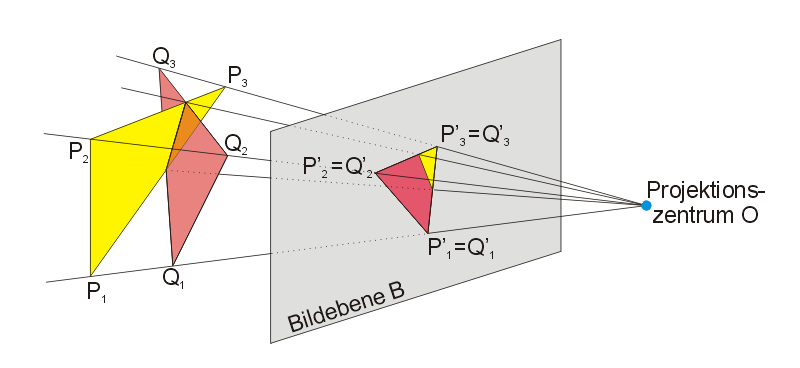
\includegraphics[width=0.6\textwidth]{images/q2_projective_geometry.jpg}
  \caption{Projection of a 3D object onto a 2D surface from a projection centre \cite{baecker_2005}.}
  \label{fig:projective_geometry}
\end{figure}

Intuitively, the projected image depends on the relative orientation of the surface and the object, and also on the distance between the projection centre and both the object and the surface. The orientation determines the projected image, and the distance defines the scale of the projection.

To capture the size of an object in a projection, since this varies with distance to the projection centre, projective geometry includes an additional coordinate, $w$, in addition to the standard Cartesian coordinates $x$ and $y$ (and $z$ in 3D space) \cite{lovell_2023b}. The additional coordinate specifies the distance between the projection and the projection centre \cite{lovell_2023b}.

Converting between projective and Cartesian coordinates in both 2D and 3D is simple \cite{lovell_2023b}:
\begin{align} \label{eqn:proj2cart}
  \text{In 2D: } (x, y, w) \longleftrightarrow \left( \frac{x}{w}, \frac{y}{w} \right) &&
  \text{In 3D: } (x, y, z, w) \longleftrightarrow \left( \frac{x}{w}, \frac{y}{w}, \frac{z}{w} \right)
\end{align}

Given the additional coordinate, $w$, if the pose of the projection centre is known, then it is possible to determine the size of the projected object.

Conversely, the projection of an object onto a surface can be calculated using a projective matrix, $P$. For the projection of a 3D object onto a 2D surface, the projective matrix has dimensions $3\times4$ \cite{lovell_2023b}, and internally captures all necessary information regarding the pose of the projection centre relative to the object.

Using projective coordinates, the projection of a point in 3D space relative to a surface and projection centre specified by some projection matrix is realised on the 2D surface as \cite{lovell_2023b}:
\begin{align} \label{eqn:projn}
  \begin{bmatrix}
    p_{11} & p_{12} & p_{13} & p_{14} \\
    p_{21} & p_{22} & p_{23} & p_{24} \\
    p_{31} & p_{32} & p_{33} & p_{34} \\
    p_{41} & p_{42} & p_{43} & p_{44} \\
  \end{bmatrix}
  \begin{bmatrix}
    x \\
    y \\
    z \\
    w \\
  \end{bmatrix}
  =
  \begin{bmatrix}
    x_i \\
    y_i \\
    w_i \\
  \end{bmatrix}
\end{align}

In the inverse direction, however, given a projection centre pose, estimating the projection matrix is a non-trivial task \cite{lovell_2023b}. For the purposes of this investigation, projection matrices are known for all projections; therefore, no determination of projection matrices is necessary.

\newpage
\subsection{Shape-From-Silhouette}

Shape-from-silhouette (SHS) is a method of 3D reconstruction using silhouettes of an object as viewed from multiple known positions \cite{lovell_2023b}. In the nomenclature of projective geometry, a silhouette is a 2D projection of an object in 3D space, formed by the intersection of the visual cone of a ``camera'' at the projection centre \cite{cheung_2005}. Using a sufficient number of silhouettes from cameras with different relative poses, the 3D object can be approximately reconstructed as the intersection of the various visual cones \cite{lovell_2023b}. This is demonstrated by Figure \ref{fig:silhouettes}.

\begin{figure}[ht]
  \centering
  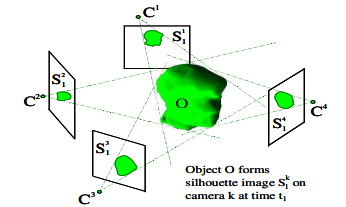
\includegraphics[width=0.5\textwidth]{images/q2_shape_from_silhouette.png}
  \caption{Silhouettes formed by the intersections of visual cones with a surface (from \cite{cheung_2005}).}
  \label{fig:silhouettes}
\end{figure}

The algorithm is programatically simple. The 3D reconstruction begins as a solid bounding box around the object of interest. Given a silhouette and an associated projection matrix, which defines the projective transformation between points in 3D space and points on the silhouette plane, each point in the reconstruction is projected onto the silhouette plane and compared with the silhouette. If the projected point lies outside the silhouette, then it is removed from the reconstruction. This is performed for all points in the reconstruction, and repeated for all available silhouettes. Once the algorithm concludes, the remaining shape is an approximate reconstruction of the original 3D object; the accuracy of the reconstruction depends on the number of silhouettes and the geometry of the object.

For example, Figure \ref{fig:shs_example} presents three SHS reconstructions of the same 3D model using an increasing number of silhouettes. The difference in reconstruction quality is evident.

\begin{figure}[ht]
  \centering
  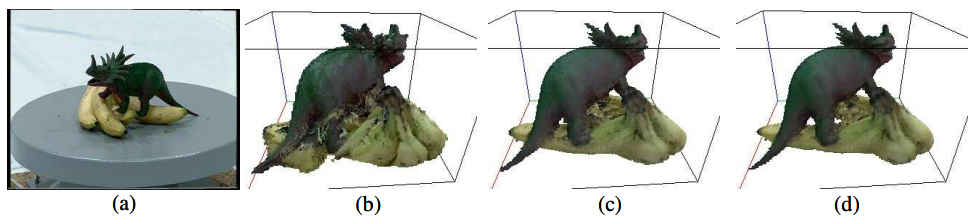
\includegraphics[width=0.8\textwidth]{images/q2_shape_from_silhouette_example.png}
  \caption{Coloured reconstructions of (a) using 6 (b), 36 (c), and 66 (d) silhouettes (from \cite{cheung_2005}).}
  \label{fig:shs_example}
\end{figure}

The advantages of SHS for 3D reconstruction include the easy availability of silhouettes, especially in an indoor environment with static cameras and controlled lighting \cite{cheung_2005}. For example, the Oxford Dinosaur dataset is derived from a single static camera capturing photographs at regular intervals of a dinosaur toy on a turntable. The colour of the photograph backgrounds makes it easy to segment a silhouette of the dinosaur.

However, SHS also has certain limitations. Foremost among these are that the quality of the reconstruction is highly dependent on the number of distinct silhouettes \cite{cheung_2005}. The method can also be sensitive to noise in segmented silhouettes \cite{lovell_2023b}. Finally, the method always produces a conservative reconstruction, and inherently cannot model convexities \cite{cheung_2005}.

\newpage
\section{Methodology}
\subsection{Silhouette Segmentation}

Before applying the shape-from-silhouette method, the colour images of the Oxford Dinosaur data set must be converted into silhouettes. This is made intentionally easy by the contrast between the foreground and background in the images. The procedure for each image follows:

\begin{enumerate}
  \item The image is converted into HSV and the hue channel is extracted.

  \item The hue image is first binarized using an experimentally-tuned lower threshold of 75.

  \item The hue image is again binarized using an experimentally-tuned upper threshold of 130.

  \item The two binarized images are combined using a logical AND to preserve the foreground regions of each.

  \item Border-connected white regions are cleared, removing noise from the black strip at the right side of the images.

\end{enumerate}

Two thresholds are used to improve the segmentation accuracy of shadowed parts of the dinosaur. The lower threshold segments the background, but also removes shadowed parts of the dinosaur. The upper threshold restores only the shadowed parts of the dinosaur. This is demonstrated in Figure \ref{fig:thresholds}.

\begin{figure}[ht]
  \centering
  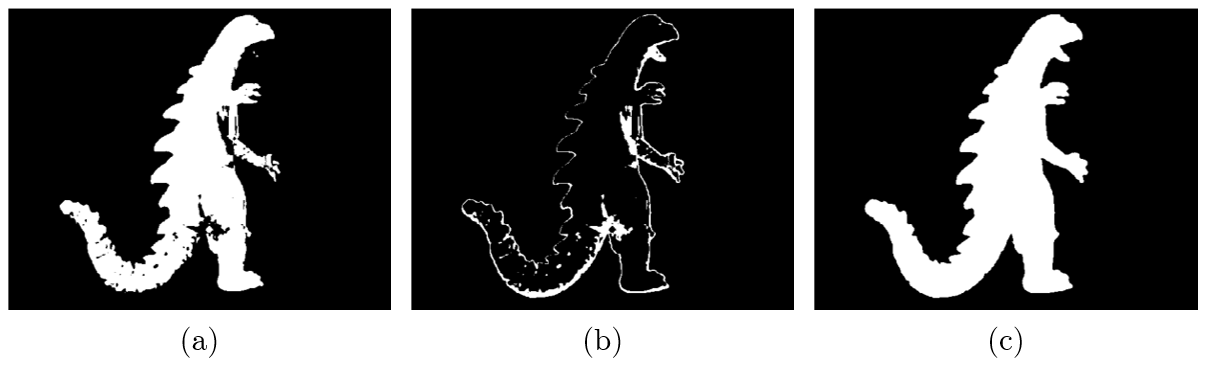
\includegraphics[width=0.7\textwidth]{images/q2_thresholds.png}
  \caption{Upper (a) and lower (b) thresholds of hue image produce a clean segmentation (c).}
  \label{fig:thresholds}
\end{figure}

\subsection{Intuitive Shape-From-Silhouette}

Following silhouette segmentation, two implementations of the SHS algorithm were attempted. The first implementation is an intuitive but slow approach based on nested for-loops. The run time of this implementation frequently exceeds 30 minutes on a reasonbly powerful desktop computer.

\begin{enumerate}
  \item A 3D tensor of size equal to the dinousaur bounding box is created. Per ``Volume.txt'', this has dimensions $271\times151\times441$ voxels; a total of approximately 18 million voxels. All voxels have an initial value of one.

  \item For each silhouette and associated projection matrix:
  \begin{enumerate}
    \item Each voxel is addressed one at a time; the voxel is constructed into a homogeoneous projective coordinate (by appending a 1) and multiplied by the projection matrix per Equation \ref{eqn:projn}, yielding a 2D projective coordinate on the plane of the silhouette.

    \item The 2D projective coordinate is converted into a Cartesian coordinate per Equation \ref{eqn:proj2cart} and rounding to the nearest integer.

    \item If the coordinate does not coincide with a point inside the silhouette, then the value of the voxel is set to zero. Voxels with a value of zero are not re-addressed in following iterations.

  \end{enumerate}
\end{enumerate}

By this process, the volume is iteratively ``carved'' from the viewpoint of each silhouette. However, the time complexity of this approach is significant. Across the 36 silhouettes, the innermost loop executes approximately 650 million runs. On a relatively powerful desktop computer, this implementation takes over 30 minutes to execute, making it a tedious process to debug mid-run failures and tune the algorithm.

\subsection{Optimised Shape-From-Silhouette}

To improve the run time speed of the SHS algorithm, a matrix-based approach is adopted based on the SpaceCarving program by Zins \cite{zins_2019}. The optimised implementation leverages the extensive matrix operation optimisations of the python package NumPy to reduce the run time to approximately 15 seconds, representing a speed improvement of over 99\%.

The steps for the optimised implementation are:
\begin{enumerate}
  \item A voxel array of all 18 million 3D projective coordinates is constructed. For example, the first entry in the array is $(-180, -80, 20, 1)$.

  \item For each silhouette and projection matrix, the projected 2D coordinates are calculated simultaneously by matrix multiplying the voxel array with the projection matrix.

  \item The 2D projective coordinates are converted to Cartesian coordinates by dividing by the scaling factor. Coordinates outside the bounds of the silhouette are discarded.

  \item The voxels are compared with the silhouette in a single step by indexing directly into the silhouette image with the projected coordinates to determine.

  \item The voxel states (filled or unfilled) for each silhouette are recorded in an array.

  \item After all silhouettes have been processed, unfilled voxels are carved away simultaneously by compressing the voxel states using a logical AND operation, which clears all voxels that are unfilled in any silhouette.

\end{enumerate}

The speed improvement derives mainly from three changes. First and second, creating an array of voxel coordinates rather than a direct representation of the volume enables fast matrix multiplication of the entire set of voxels at once with the projection matrix. This removes all three nested for-loops, offering a significant performance improvement as a result of NumPy's C API. Third, indexing directly into the silhouette to determine filled and unfilled voxel states is significant faster than iterating over the voxels.

The sole caveat of the optimised method is that in exchange for the significant performance improvement, the intuition of the SHS algorithm is somewhat obscured.

\newpage
\section{Results}

Figure \ref{fig:dino_views} presents four new views of the dinosaur as reconstructed using the SHS algorithm and viewed using the ParaView 5.11.1 software \cite{kitware_2023}.

\begin{figure}[ht]
  \centering
  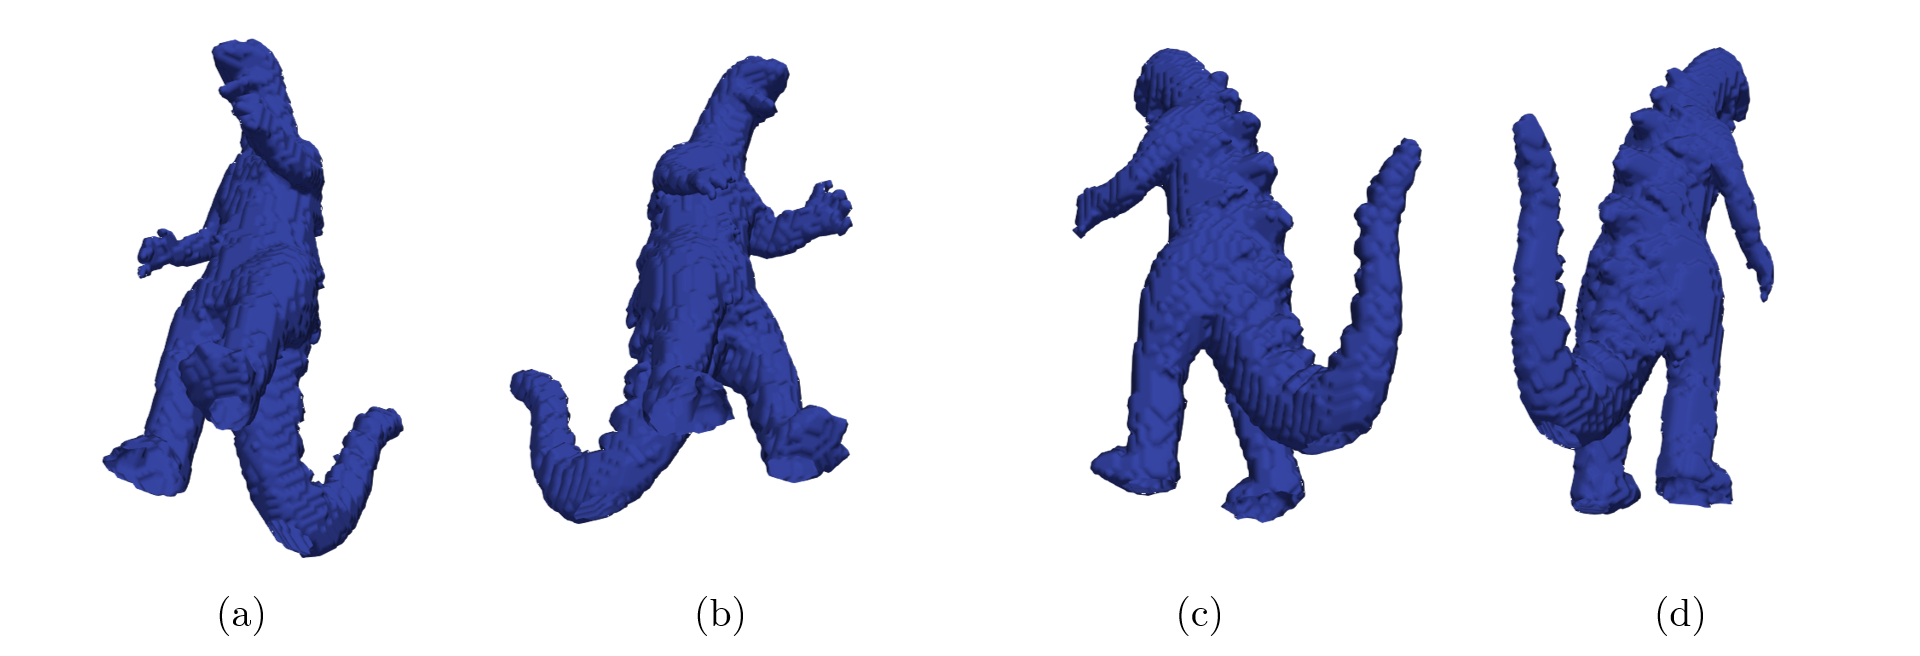
\includegraphics[width=0.9\textwidth]{images/q2_dino_views.png}
  \caption{Four views of the reconstructed dinosaur, not coinciding with data set views.}
  \label{fig:dino_views}
\end{figure}

\newpage
\section{Discussion}

This report has presented an implementation of the shape-frome-silhouette (SHS) algorithm, and applied it to reconstruct a model of the Oxford Dinosaur from a data set of 36 images and projection matrices. The solution successfully reconstructs the dinosaur to an expected degree of accuracy, and demonstrates advantages and disadvantages of the SHS algorithm.

Prime among the advantages of the SHS algorithm is the easy availability of silhouettes, especially in a controlled environment \cite{cheung_2005}. This is demonstrated by the high segmentation accuracy achievable on the Oxford Dinosaur data set, enabled by consistent and high quality lighting and a background chosen to contrast strongly with the dinosaur foreground. The segmentated first image is provided as an example in the Methodology section.

On the other hand, this advantage arguably only compensates for the simultaneous sensitivity of the algorithm to segmentation accuracy \cite{lovell_2023b}. This sensitivity arises from the practice of clearing voxels which appear empty in any silhouette. As a result, if any silhouette is improperly segmented, parts of the model may erroneously appear empty and be cleared, which by design of this particular implementation cannot be rectified by any subsequent process.

A remedy to this, as implemented by the SpaceCarving implementation of Zins \cite{zins_2019}, is to instead capture a count of the number of viewpoints perceiving each voxel as non-empty. If this count exceeds some threshold, then the voxel is considered non-empty. This is a conservative approach to SHS, which affords some tolerance to segmentation errors. However, the accuracy of the reconstruction is notably inferior, resulting in erroneous protrusions when applied to the Oxford Dinosaur problem.

A further limitation, conceivably greater than just discussed, is that the quality of the reconstruction is highly dependent on the number of distinct silhouettes \cite{cheung_2005}. This is demontrated by Figure \ref{fig:shs_example} from Cheung et. al \cite{cheung_2005}, and a similar example is presented by Figure \ref{fig:bad_reconstruction} for the Oxford Dinosaur model.

\begin{figure}[ht]
  \centering
  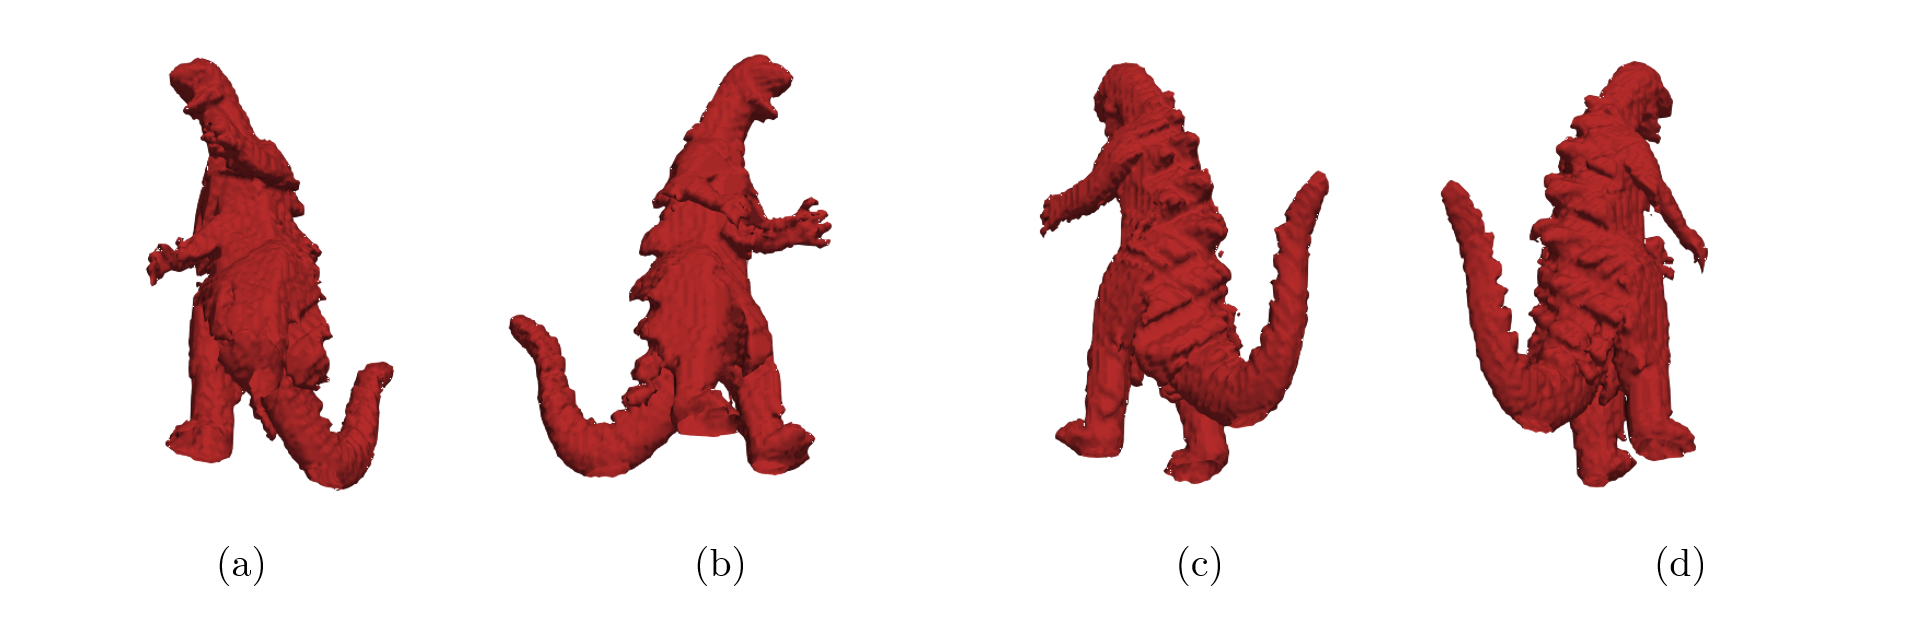
\includegraphics[width=0.9\textwidth]{images/q2_bad_reconstruction.png}
  \caption{Reconstruction of the Oxford Dinosaur using only six silhouettes.}
  \label{fig:bad_reconstruction}
\end{figure}

Figure \ref{fig:bad_reconstruction} presents the SHS reconstruction of the Oxford Dinosaur using only every sixth silhouette; the result may be compared to Figure \ref{fig:dino_views} and the significant difference observed. This limitation is inherent to the SHS method, and is particularly consequential for scenarios where a practitioner may have access only to a limited existing set of images or silhouettes. This may be likely, for example, in medical imaging applications. If the silhouettes are further imperfectly segmented, then the SHS reconstruction will have a very limited quality.

\section{Conclusion}

In summary, this report presents an implementation of the shape-from-silhouette algorithm, and the result it achieves in reconstructing the Oxford Dinosaur. The result demonstrates advantages and limitations of the shape-from-silhouette algorithm. Notably, a discussion is founded surrounding the sensitivity of the algorithm to segmentation accuracy, and the necessity of a sufficient number of distinct silhouettes.
